\documentclass{ncc}
\usepackage[utf8]{inputenc}
\usepackage[russian]{babel}
\usepackage[T2A]{fontenc}
\usepackage{amssymb}
\usepackage{amsmath}
\usepackage{pscyr}
\usepackage{graphicx}
\usepackage{listings}
\usepackage[colorlinks,linkcolor=black,urlcolor=blue]{hyperref}

\lstloadlanguages{C++}
\lstset{
language=C++,
extendedchars=\true, %Чтобы русские буквы в комментариях были
keepspaces=true,
inputencoding=utf8,
breaklines,
columns=fullflexible,
flexiblecolumns,
numbers=left,
numberstyle={\footnotesize},
commentstyle=\it,
stringstyle=\bf,
belowcaptionskip=5pt }


\title{Ограниченная аналитическая функция}

\begin{document}
\maketitle

Продолжаем цикл <<простенько и со вкусом>>. Сегодня рассмотрим задачу от всё того же Серёжи, которая мучила меня пару месяцев. Требуется доказать, что если аналитическая на всей комплексной плоскости функция ограничена (\(|f(z)| < M\)), то она всюду постоянна.

Начнём с понятия аналитической функции. Если мы имеем всюду аналитическую функцию \( f(z) \), то она дифференцируема на всей комплексной плоскости. Поэтому малая окрестность любой точки плоскости \( z_0 \) конформно отображается на окрестность точки \( w_0 = f(z_0) \):
\[
    f(z_0 + \varepsilon) = w_0 + f^\prime(z_0)\varepsilon + o(\varepsilon),
\]
растягиваясь при этом в \( |f^\prime(z_0)| \) раз.

Доказывать будем от противного. Итак, пусть у нас есть аналитическая функция \( f(z) \ne \mathrm{const} \), которая вдобавок ограничена: \( |f(z)| < M \). Если она ограничена, то в некоторой точке \( a \) её модуль \(|f(z)|\) достигает своего наибольшего значения. Как мы уже знаем, функция \( f(z) \) переводит окрестность точки \( a \) в окрестность точки \( f(a) \), как показано на рисунке ниже.

\begin{figure}[h]
    \center
    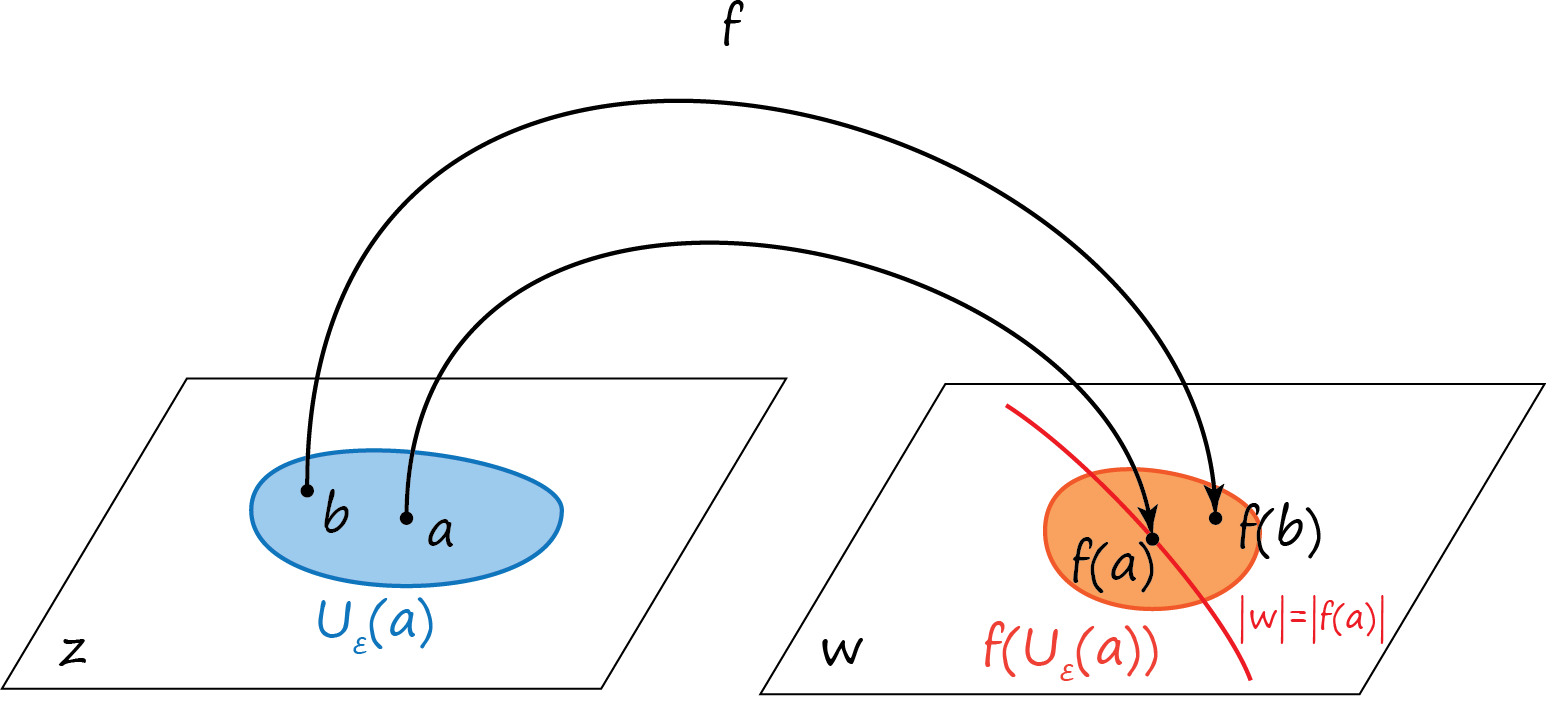
\includegraphics[width=0.6\textwidth]{2016-05-27-analytic-function.png}
\end{figure}

Как мы видим, в окрестности точки \( f(a) \) найдётся точка \( w = f(b) \), для которой \( |f(b)| > |f(a)| \). Но это противоречит нашему допущению о наибольшем значении \( |f(z)| \). Следовательно, \( f(z) = \mathrm{const} \).
\end{document}
